\newpage
\section{Реализация}
\label{sec:Realization}

 \fxnote{} 

\subsection{Обработка данных для модели}
\label{subsec:Parser}

 Текущий датасет содержит множество полей, где каждая запись соответствует определенной действия, выполненной пользователем в одном из репозиториев. В частности, существует столбец <<event\_type>>, который описывает различные операции. Для данной работы нас интересуют следующие операции: <<CommitCommentEvent>> (добавление коммита с комментарием), <<ForkEvent>> (создание форка репозитория), <<IssuesEvent>> (добавление обсуждения), <<PullRequestEvent>> (создание запроса на включение изменений), и <<WatchEvent>> (добавление звезды к проекту). В контексте работы с проектами, необходимо сгруппировать выполненные операции для каждого проекта. Следовательно, с использованием запросов можно получить информацию о названии проекта (репозитория) и количестве звезд, форков и других характеристик, связанных с данным репозиторием.

 После установления ключевых параметров, необходимо определить цель использования этих данных и методы их получения. В рамках данного исследования, нацеленного на разработку системы классификации проектов на платформе GitHub в зависимости от их популярности, имеется неотъемлемая потребность в доступе к данным из базы данных. Эти данные из датасета GitHub будут использованы для обучения модели классификации, её оценки и настройки. Оценка модели позволит установить, насколько успешно она способна разделять проекты на популярные и непопулярные.

Исходными данными для этой работы служит статья о наборе данных GitHub~\cite{clickHouse}, содержащем информацию о всех событиях на этой платформе с 2011 года и насчитывающем более трех миллиардов записей. Данный набор данных был загружен в ClickHouse, который представляет собой открытую систему управления базами данных, специально разработанную для эффективного анализа и хранения больших объемов информации. Одной из важных особенностей этой технологии является её акцент на аналитических задачах, что обеспечивает возможность проведения сложных анализов данных.

Текущий набор данных GH Archive представлен как в формате ClickHouse Native с объемом более 70 ГБ, так и в альтернативном формате, разделенном табуляцией, с объемом 85 ГБ. Учитывая, что данные из этого набора нужны лишь для однократного обучения модели без необходимости долгосрочного доступа ко всей базе данных, было принято решение извлекать такие объемы данных из других хранилищ данных, а не с физических устройств.

Помимо того, для демонстрации работы с общедоступными данными ClickHouse существует веб-страница, способная обрабатывать SELECT-запросы и предоставлять обширный объем информации. Все данные, полученные таким образом, являются полными, вследствие чего было определено осуществлять извлечение результатов запросов из HTML-страницы.

В силу того, что данные из датасета ClickHouse было решено получать из веб-приложения, необходимо разработать способ, которым можно корректно их преобразовать.

Для этой цели был разработан класс, содержащий несколько методов. Самый важный метод позволяет извлекать данные из разметки страны формата html. Этот метод принимает параметр, который определяет желаемый объем данных для извлечения. 

Данная функция имитирует взаимодействие с веб-страницей, используя библиотеку Selenium WebDriver для управления браузером. Он создает виртуальное окружение браузера, отправляет запрос. После ожидания получения результата в течение 10 секунд данные извлекаются из таблицы на веб-странице с использованием библиотеки Beautiful Soup, предназначенной для анализа HTML-файлов. 

Исследователи из Федерального университета Минас-Жерайс, Бразилия представили результаты своей работы, в которой они анализировали прогноз популярности проектов на GitHub~\cite{BorgesHV16}. Вследствие того, что GitHub является динамичной платформой, на которой постоянно появляются новые проекты, технологии и тренды, анализ данных за последние 5-8 лет позволит  учесть актуальные тенденции в мире разработки программного обеспечения. Использование данных за это время позволит увидеть динамику изменений в популярности проектов и научиться предсказывать будущие тренды. 

Кроме того, важно учитывать только уникальные вклады от каждого пользователя потому, что это позволит избежать искажений в данных, вызванных многократным участием одного пользователя. Также уникальные авторы коммитов обеспечат разнообразие данных, позволяя модели учитывать вклад различных участников проекта при определении его популярности. В результате было решено использовать данные за последние 8 лет и учитывать данные об уникальных авторах коммитов.

Полученные данные могут быть представлены в различных форматах, таких как JSON, CSV и другие. Для работы в дальнейшем будет использоваться формат CSV для обработки. Так, было получено около трехсот тысяч данных.

\subsection{Обучение модели}
\label{subsec:Learning}

Для решения задачи классификации на основе данных платформы GitHub был разработан класс GitHubClassifier. Этот класс содержит несколько методов, предназначенных для обработки данных, обучения моделей и оценки их производительности.

Класс инициализируется путем загрузки данных из CSV-файла и предварительной обработки. Данные подвергаются масштабированию с использованием метода MinMaxScaler из библиотеки sklearn.preprocessing, что позволяет привести значения признаков к одному масштабу.

Для обучения моделей классификации, таких как RandomForestClassifier и GradientBoostingClassifier из библиотеки sklearn.ensemble, используются подготовленные данные. Обученные модели позволяют прогнозировать классы новых данных и оценивать их точность с помощью методов count\_f1, count\_precision и count\_recall, возвращающих значения F1-меры, точности и полноты соответственно.

Также предоставлены методы для вывода матрицы ошибок (get\_confusion\_matrix) в форме графика (plot\_confusion\_matrix), сохранения и загрузки обученных моделей (save\_model и load\_model). Эти методы обеспечивают анализ результатов классификации и позволяют использовать обученные модели для прогнозирования классов новых данных.

\subsection{Графический интерфейс (веб-страница)}
\label{subsec:gui}

В качестве первичного графического интерфейса и возможности отображения работы с моделью было выбрано веб-приложение, которое написано на популярном фреймворке Flask. 

На главной странице отображается форма (рис.~\ref{ris:form-data}) для добавления параметров репозитория, что необходимы для определения модели ранга популярности. 

\begin{center}
    \begin{figure}[H]
        \center{\includegraphics[width=0.4\linewidth]{image}}
        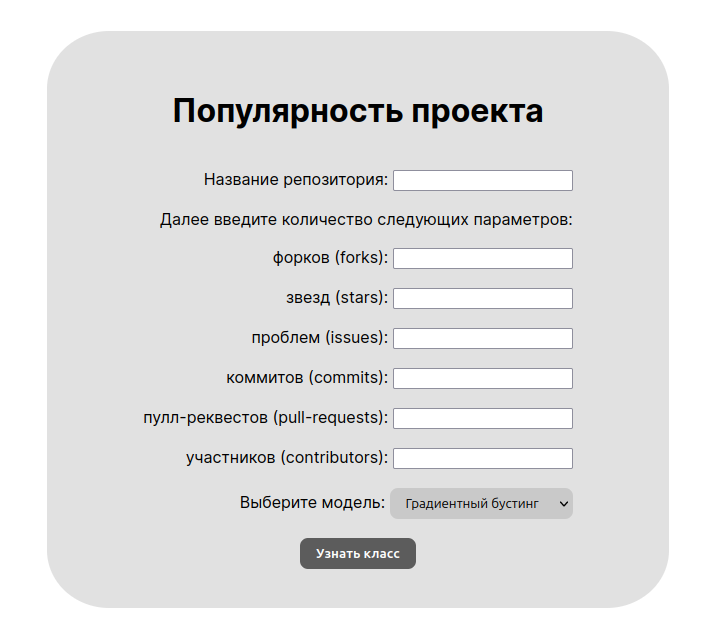
\includegraphics[scale=0.5]{pic/form-data.png}
        \caption{Форма для ввода данных}
        \label{ris:form-data}
    \end{figure}
\end{center}
\vspace{1.5em}

Кроме того, можно выбрать модель, на базе которой будет определен класс популярности проекта. После получения данные проходят обработку, и открывается страницу, на которой отображен результат определения полученного ранга с перечислением того, какие данные были отправлены (рис.~\ref{ris:result-data})

\begin{center}
    \begin{figure}[H]
        \center{\includegraphics[width=0.4\linewidth]{image}}
        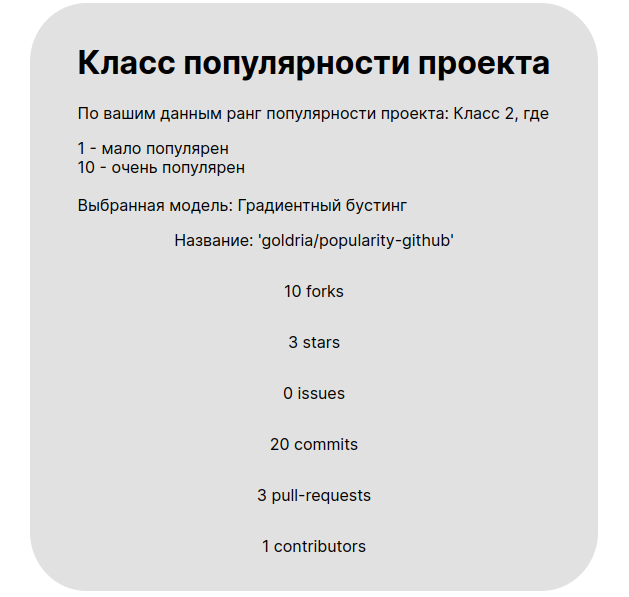
\includegraphics[scale=0.5]{pic/result-data.png}
        \caption{Форма для ввода данных}
        \label{ris:result-data}
    \end{figure}
\end{center}
\vspace{1.5em}